\section{Introduzione}
Alla base di questa tesi vi è il manipolatore PKM (\textit{parallel kinematic manipulator}). Un manipolatore parallelo è un sistema meccanico che utilizza "catene" seriali per supportare un \textit{end-effector}, ogni catena solitamente è corta, semplice e di conseguenza può essere rigida rispetto a movimenti non voluti rispetto ad un manipolatore seriali. La movimentazione e la flessibilità di un \textit{joint} è vincolata dall'effetto delle altre catene, questo rende il manipolatore rigido rispetto alle sue componenti.
\\L'obiettivo di questa tesi riguarda la modellazione teorica e pratica del manipolatore, in particolare l'interesse risiede nella movimentazione andando a generare ed eseguire traiettorie bidimensionali e tridimensionali
\begin{figure}[ht]
\begin{center}
    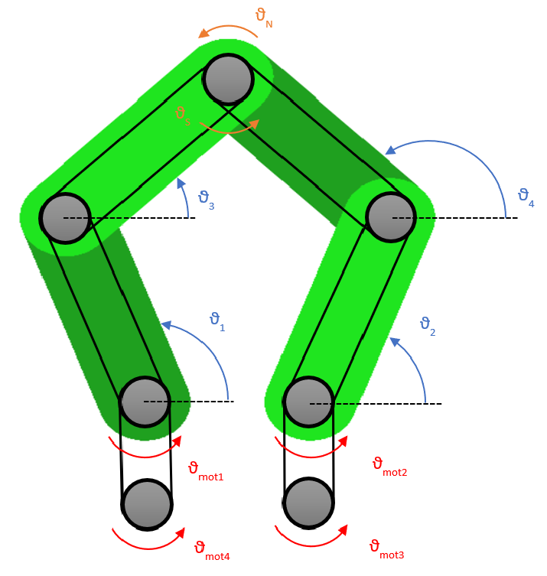
\includegraphics[scale=0.7]{Immagini/Robot1.png}
    \caption{Robot PKM}
\end{center}
\end{figure}
Escludendo l'introduzione, la tesi è articolata sette capitoli: nel secondo capitolo viene presentata l'analisi cinematica del manipolatore, in particolare verranno analizzate sia cinematica diretta che inversa, nel terzo capitolo si parla di dinamica, punti di singolarità e manipolabilità del robot; il quarto capitolo mostra la modellazione dell'\textit{end-effector}, nel nostro caso la vite; il quinto capitolo va a presentare tutte le tecnologie implementate a livello pratico, e per concludere nel sesto capitolo viene presentato il sistema reale, includendo la struttura, l'implementazione, il sistema di controllo ed i problemi riscontrati con relative soluzioni; nel settimo capitolo, infine, verranno esposte le conclusioni, grazie ad un confronto ottenuto dai risultati teorici e quelli pratici.
\subsection{Software utilizzati}
In questa sezione andremo ad introdurre i programmi software utilizzati per la modellazione teorica del manipolatore, in particolare parleremo di Matlab e Adams.
\subsubsection{Matlab}
Matlab, abbreviazione di \textit{Matrix Laboratory}, è una piattaforma di calcolo ottimizzata nella risoluzione di problemi tecnici. 
Matlab è un linguaggio ad alte prestazione per la computazione tecnica, integra computazione, visualizzazione e programmazione in un ambiente di facile utilizzo dove i problemi e le soluzioni vengono espressi mediante una notazione matematica, gli utilizzi tipici riguardano: matematica e computazione, sviluppo di algoritmi, modellazione, simulazione, prototipazione, analisi dei dati, intelligenza artificiale. La base di matlab è un vettore che non ha bisogno di dimensioni, in questo modo permette la risoluzione di molti problemi di computazione, specialmente quelli in formulazione vettoriale e matriciale velocemente, senza dover ricorrere all'utilizzo di linguaggi come il C. Matlab inoltre possiede delle \textit{toolbox} ovvero moduli aggiuntivi che permettono di specializzarsi in un campo, in particolare sono insieme di funzioni MATLAB che estendono l'ambiente, permettendogli di risolvere particolari classi di problemi, esempi di moduli sono reti neurali, processamento di segnali, sistemi di controllo.
\\Nel nostro caso abbiamo definito il modello teorico del robot, abbiamo poi calcolato cinematica, dinamica e punti di singolarità, nei capitoli successivi verranno mostrate le operazioni fatte. 
\subsubsection{Adams}
Adams è un software utilizzato nel campo della dinamica \textit{multibody}, in particolare nell'analisi dei modelli, infatti dopo che è stato progettato un modello può essere importato in adams ed è possibile fare analisi, simulazioni e validazioni, andando quindi a simulare la fisica del mondo reale. Adams è anche ottimizzato per problemi di grandi dimensioni.
\\Il software ha una GUI completa, infatti consente anche di disegnare direttamente il modello nello spazio tridimensionale o di importare file come STEP e IGS. I \textit{joint} possono essere aggiunti tra due corpi per vincolare il loro movimento, inoltre al sistema possono essere passati input come velocità, forze e condizioni iniziali. Adams simula il comportamento del sistema al variare del tempo, consente anche l'animazione e la computazione di proprietà come le forze, le inerzie e le accelerazioni, è anche possibile nel sistema includere elementi complessi dinamicamente come per esempio molle, corpo flessibili, contatto tra corpi.
É inoltre possibile esportare tutti i dati in formato tabellare per fare analisi successive. 
\\Per quanto riguarda il nostro caso, abbiamo utilizzato Adams per modellare il robot, assegnargli le coppie e confrontare i valori della cinematica e dinamica con quelli ottenuti da Matlab, nei capitoli successivi verrà presentato un confronto tra questi dati.